\documentclass{beamer}

\mode<presentation>
{
    \usetheme{rwthsimple}
    \setbeamercovered{transparent = 0}
}

\setbeamertemplate{section in toc shaded}[default][30]
\setbeamertemplate{subsection in toc shaded}[default][30]

% \pgfplotsset{compat=1.9}

\title{}
\author{}
\date{}

\newcommand\blfootnote[1]{%
    \begingroup
    \renewcommand\thefootnote{}\footnote{#1}%
    \addtocounter{footnote}{-1}%
    \endgroup
}

% \usepackage[scaled]{helvet} % Helvetica
%\usepackage[scaled]{uarial} % Arial
\usepackage{subcaption}
\renewcommand*\familydefault{\sfdefault} %% Only if the base font of the document is to be sans serif
\usepackage[T1]{fontenc}

\usepackage{biblatex}
\usepackage{tikz}
\usepackage[font=scriptsize,labelformat=empty]{caption}
\usepackage{xcolor}
\usepackage{scrextend}
\changefontsizes{14pt}

% https://tex.stackexchange.com/questions/21741/how-do-i-change-footnote-font-size-in-beamer-presentation
\let\oldfootnotesize\footnotesize
\renewcommand*{\footnotesize}{\oldfootnotesize\tiny}

% https://tex.stackexchange.com/questions/133955/beamer-how-to-place-images-behind-text-z-order
\makeatletter
\newbox\@backgroundblock
\newenvironment{backgroundblock}[2]{%
  \global\setbox\@backgroundblock=\vbox\bgroup%
    \unvbox\@backgroundblock%
    \vbox to0pt\bgroup\vskip#2\hbox to0pt\bgroup\hskip#1\relax%
}{\egroup\egroup\egroup}
\addtobeamertemplate{background}{\box\@backgroundblock}{}
\makeatother

\begin{document}
{\color{RWTHgrey}
	\begin{frame}[t]{}{}%
		\vfill
    		\begin{center}
    			{\LARGE Creative Applications of Deep\\[2px] Learning with Tensorflow}\\[6px]
    			{\Large\color{RWTHorange} David Stutz}\\[6px]
    			{\large Final Project}
    		\end{center}
    		\vfill
	\end{frame}
	\begin{frame}[t]{}{}%
		\vfill
    		\begin{center}
    			{\Large This project isn't creative, though ...}
    		\end{center}
    		\pause
    		\begin{center}
    			{\Large I was interested in different activation}\\[6px]
    			{\Large functions, initialization schemes}\\[6px]
    			{\Large and batch normalization.}
    		\end{center}
    		\vfill
	\end{frame}
	\begin{frame}[t]{}{}%
		\vfill
		\begin{center}
    			{\Large Dataset: MNIST}\\[6px]
    			{\Large Code: \url{davidstutz.de} (coming soon)}
    		\end{center}
    		\pause
    		\begin{center}
    			{\Large Architecture}\\[6px]
    			{\large $(\text{conv} - \text{act} - \text{pool} - \text{norm})^L$}\\[6px]
    			{\large $- \text{fc} - \text{act} - \text{norm} - \text{fc} - \text{softmax}$}
    		\end{center}
    		\vfill
	\end{frame}
	\begin{frame}[t]{}{}%
		\vfill
    		\begin{center}
    			{\Large Visualizing accuracies, activations}\\[6px]
    			{\Large and weights during training.}
    		\end{center}
    		\pause
    		\begin{center}
    			{\large Plots show average and standard}\\[6px]
    			{\large deviation over 5 repetitions.}
    		\end{center}
    		\vfill
	\end{frame}
	
	% SoftSign Heuristic
	\begin{frame}[t]{}{}%
		\vfill
		\begin{center}
			{$L = 4$ / Initialization: heuristic / Activation: softsign / Normalization: none}
		\end{center}
    		\begin{figure}
    			\centering
    			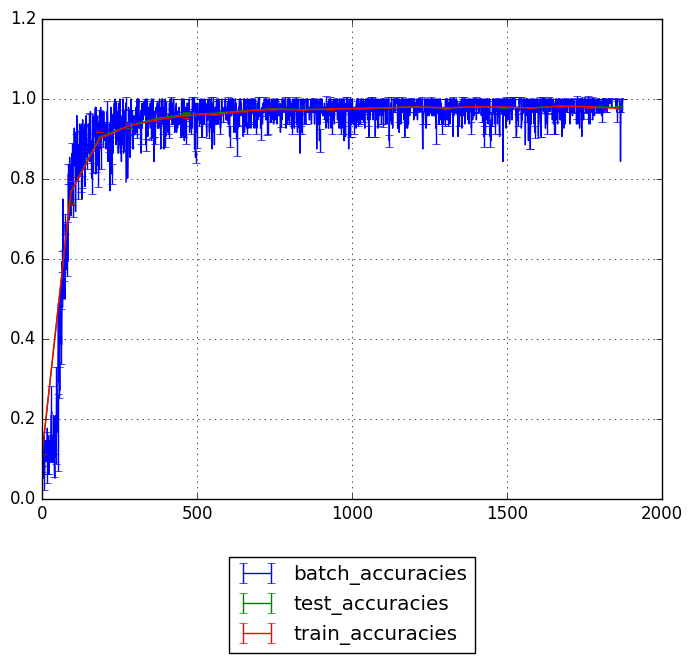
\includegraphics[scale=0.4]{gfx/l4b32_softsign_heuristic_identity_cnn_accuracies}
    		\end{figure}
    		\vfill
	\end{frame}
	\begin{frame}[t]{}{}%
		\vfill
		\begin{center}
			{$L = 4$ / Initialization: heuristic / Activation: softsign / Normalization: none}
		\end{center}
    		\begin{figure}
    			\centering
    			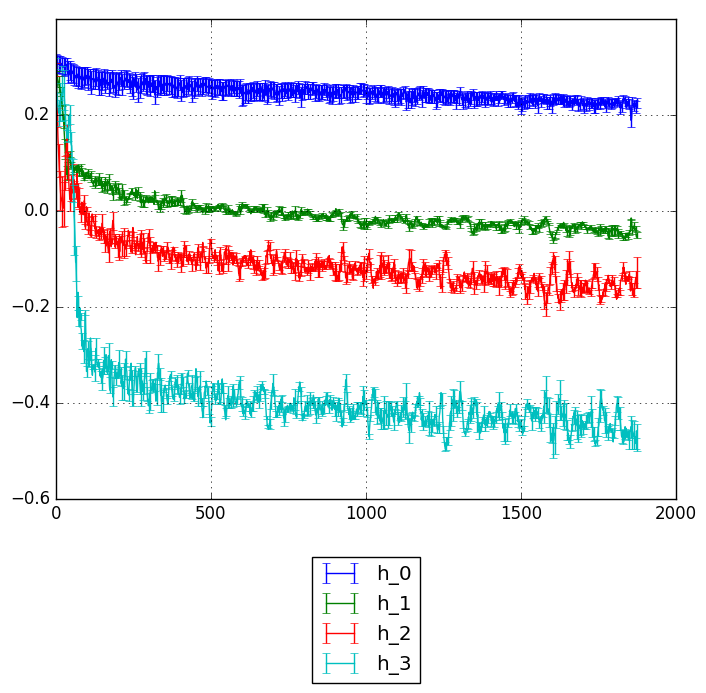
\includegraphics[scale=0.4]{gfx/l4b32_softsign_heuristic_identity_cnn_activations}
    		\end{figure}
    		\vfill
	\end{frame}
	\begin{frame}[t]{}{}%
		\vfill
		\begin{center}
			{$L = 4$ / Initialization: heuristic / Activation: softsign / Normalization: none}
		\end{center}
    		\begin{figure}
    			\centering
    			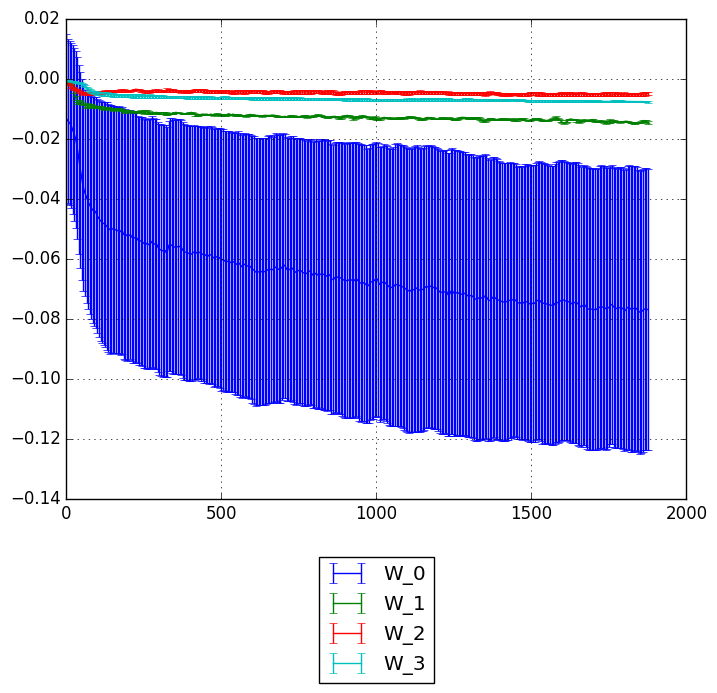
\includegraphics[scale=0.4]{gfx/l4b32_softsign_heuristic_identity_cnn_weights}
    		\end{figure}
    		\vfill
	\end{frame}
	
	% SoftPlus
	\begin{frame}[t]{}{}%
		\vfill
		\begin{center}
			{$L = 4$ / Initialization: heuristic / Activation: softplus / Normalization: none}
		\end{center}
    		\begin{figure}
    			\centering
    			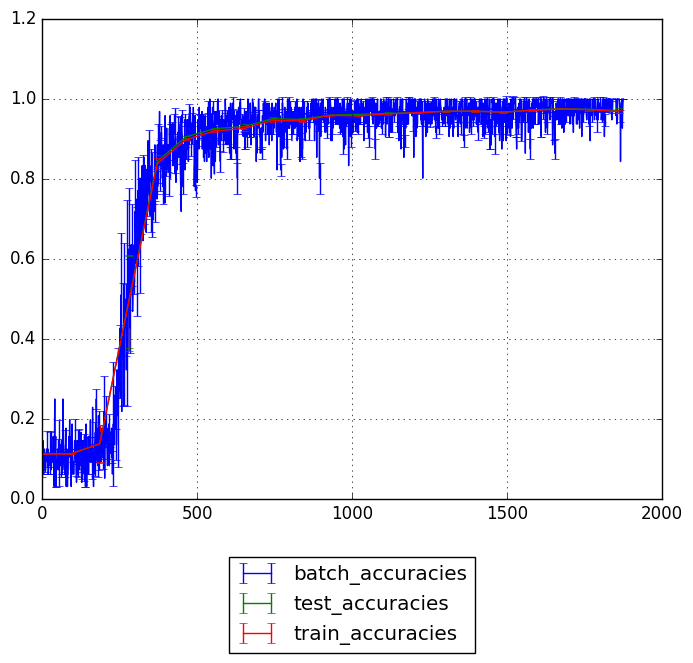
\includegraphics[scale=0.4]{gfx/l4b32_softplus_heuristic_identity_cnn_accuracies}
    		\end{figure}
    		\vfill
	\end{frame}
	\begin{frame}[t]{}{}%
		\vfill
		\begin{center}
			{$L = 4$ / Initialization: heuristic / Activation: softplus / Normalization: none}
		\end{center}
    		\begin{figure}
    			\centering
    			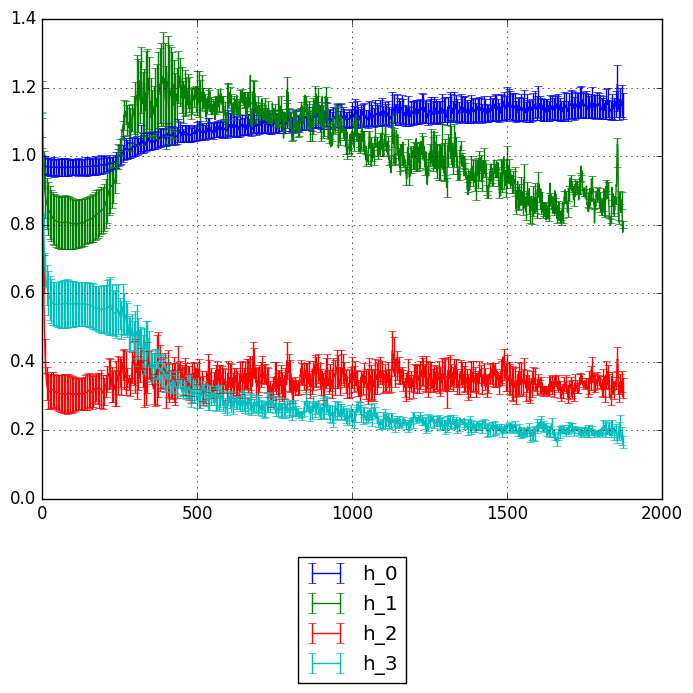
\includegraphics[scale=0.4]{gfx/l4b32_softplus_heuristic_identity_cnn_activations}
    		\end{figure}
    		\vfill
	\end{frame}
	\begin{frame}[t]{}{}%
		\vfill
		\begin{center}
			{$L = 4$ / Initialization: heuristic / Activation: softplus / Normalization: none}
		\end{center}
    		\begin{figure}
    			\centering
    			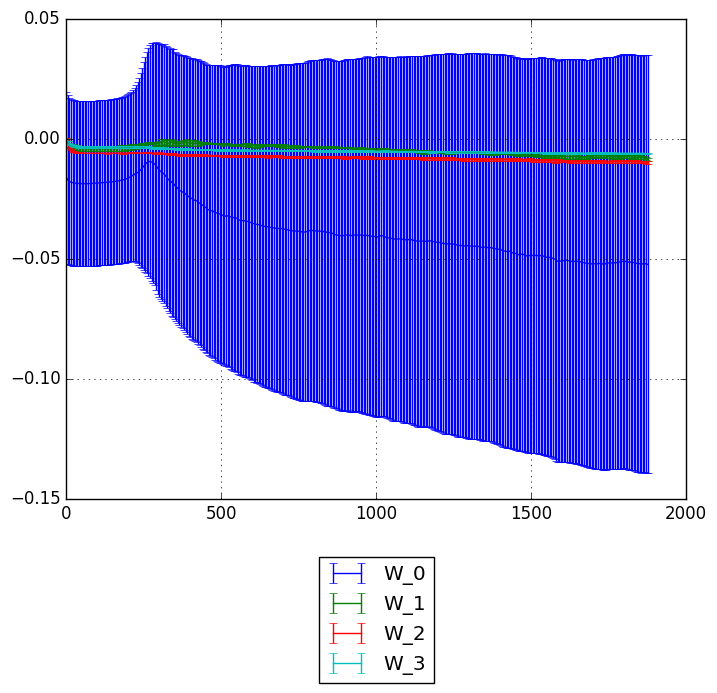
\includegraphics[scale=0.4]{gfx/l4b32_softplus_heuristic_identity_cnn_weights}
    		\end{figure}
    		\vfill
	\end{frame}
	
	% TanH
	\begin{frame}[t]{}{}%
		\vfill
		\begin{center}
			{$L = 4$ / Initialization: heuristic / Activation: tanh / Normalization: none}
		\end{center}
    		\begin{figure}
    			\centering
    			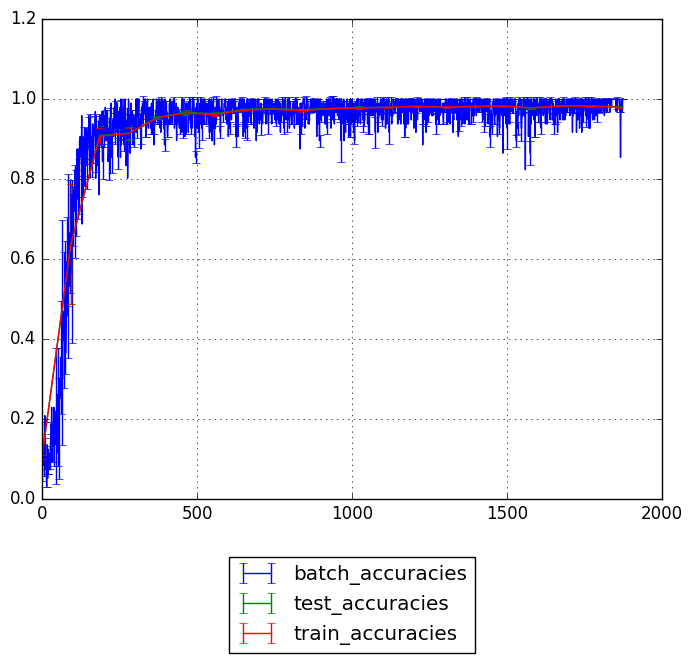
\includegraphics[scale=0.4]{gfx/l4b32_tanh_heuristic_identity_cnn_accuracies}
    		\end{figure}
    		\vfill
	\end{frame}
	\begin{frame}[t]{}{}%
		\vfill
		\begin{center}
			{$L = 4$ / Initialization: heuristic / Activation: tanh / Normalization: none}
		\end{center}
    		\begin{figure}
    			\centering
    			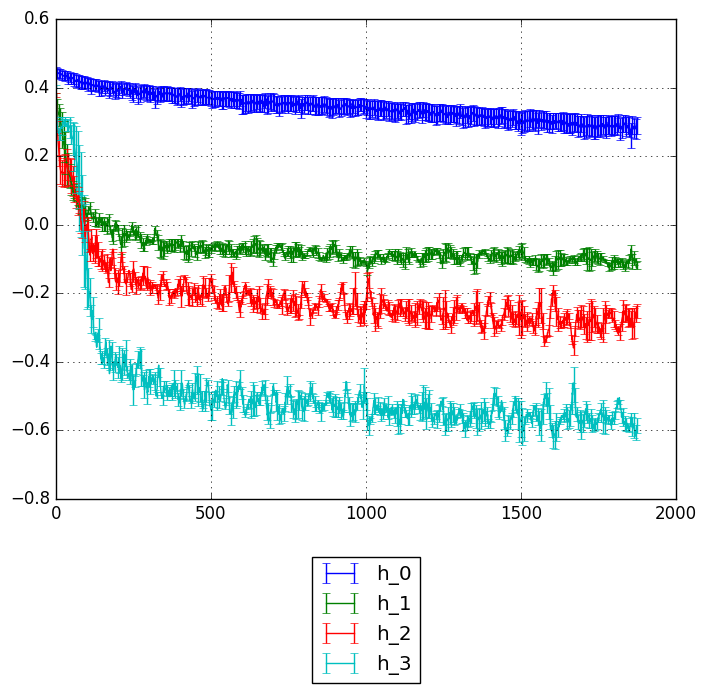
\includegraphics[scale=0.4]{gfx/l4b32_tanh_heuristic_identity_cnn_activations}
    		\end{figure}
    		\vfill
	\end{frame}
	\begin{frame}[t]{}{}%
		\vfill
		\begin{center}
			{$L = 4$ / Initialization: heuristic / Activation: tanh / Normalization: none}
		\end{center}
    		\begin{figure}
    			\centering
    			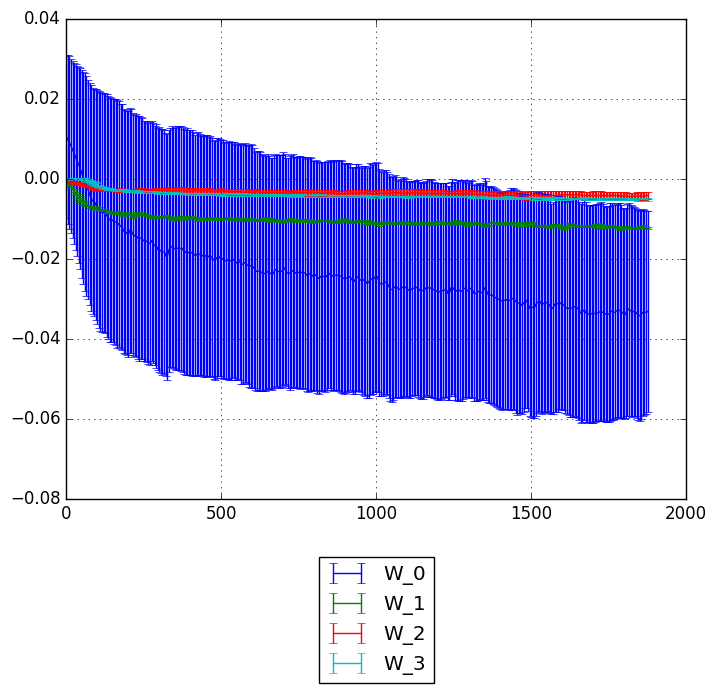
\includegraphics[scale=0.4]{gfx/l4b32_tanh_heuristic_identity_cnn_weights}
    		\end{figure}
    		\vfill
	\end{frame}
	
	% ReLU
	\begin{frame}[t]{}{}%
		\vfill
		\begin{center}
			{$L = 4$ / Initialization: heuristic / Activation: relu / Normalization: none}
		\end{center}
    		\begin{figure}
    			\centering
    			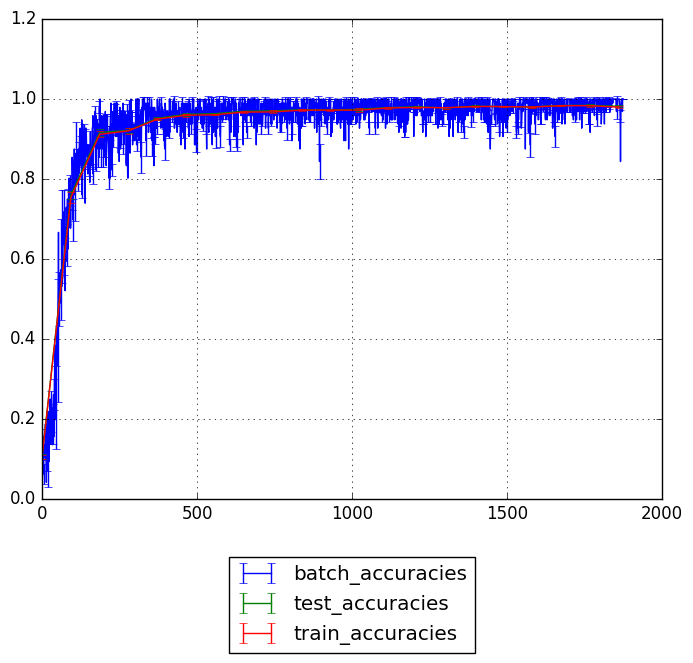
\includegraphics[scale=0.4]{gfx/l4b32_relu_heuristic_identity_cnn_accuracies}
    		\end{figure}
    		\vfill
	\end{frame}
	\begin{frame}[t]{}{}%
		\vfill
		\begin{center}
			{$L = 4$ / Initialization: heuristic / Activation: relu / Normalization: none}
		\end{center}
    		\begin{figure}
    			\centering
    			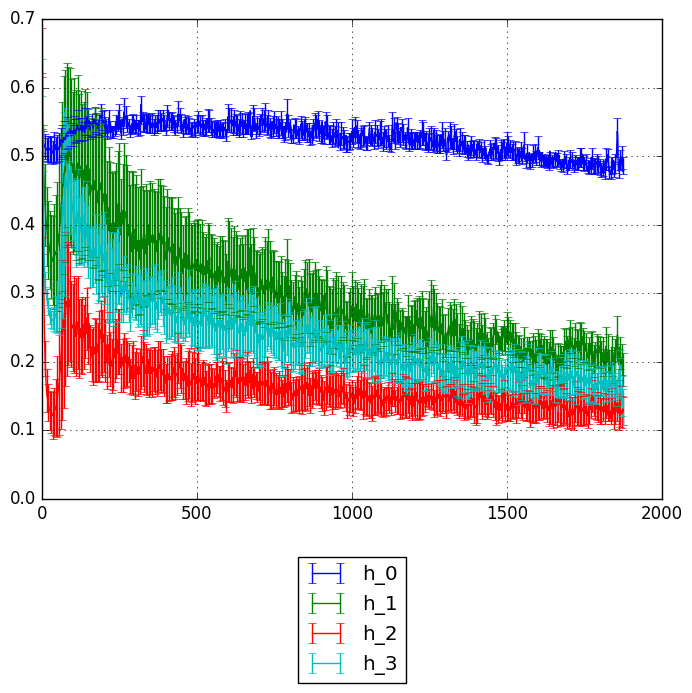
\includegraphics[scale=0.4]{gfx/l4b32_relu_heuristic_identity_cnn_activations}
    		\end{figure}
    		\vfill
	\end{frame}
	\begin{frame}[t]{}{}%
		\vfill
		\begin{center}
			{$L = 4$ / Initialization: heuristic / Activation: relu / Normalization: none}
		\end{center}
    		\begin{figure}
    			\centering
    			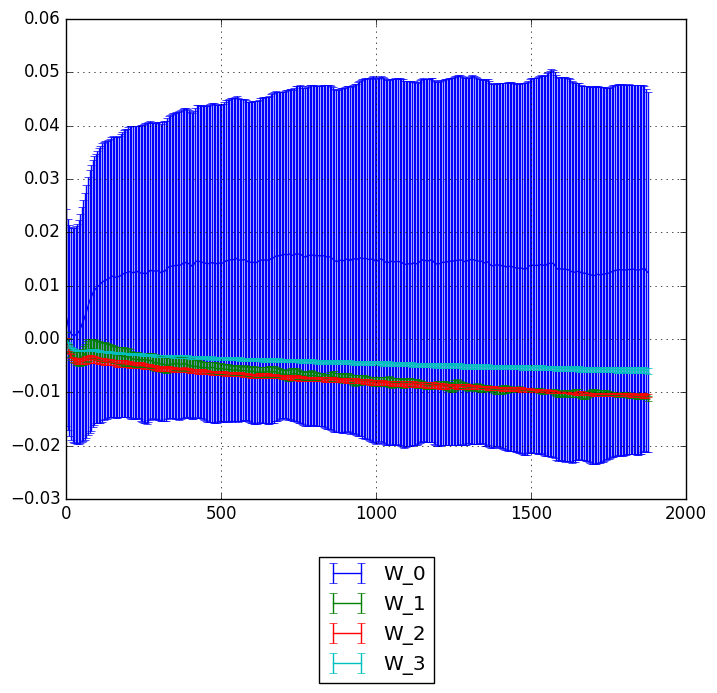
\includegraphics[scale=0.4]{gfx/l4b32_relu_heuristic_identity_cnn_weights}
    		\end{figure}
    		\vfill
	\end{frame}
	
	% ReLU + Xavier
	\begin{frame}[t]{}{}%
		\vfill
		\begin{center}
			{$L = 4$ / Initialization: xavier / Activation: relu / Normalization: none}
		\end{center}
    		\begin{figure}
    			\centering
    			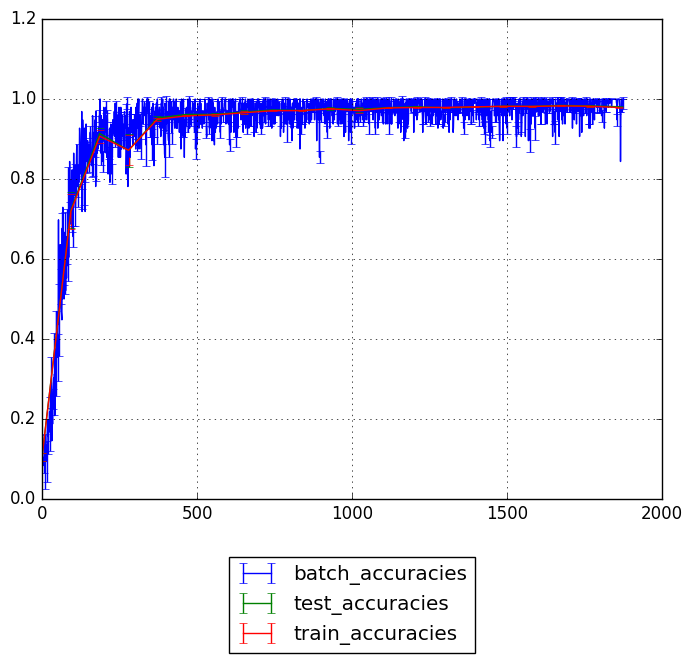
\includegraphics[scale=0.4]{gfx/l4b32_relu_xavier_identity_cnn_accuracies}
    		\end{figure}
    		\vfill
	\end{frame}
	\begin{frame}[t]{}{}%
		\vfill
		\begin{center}
			{$L = 4$ / Initialization: xavier / Activation: relu / Normalization: none}
		\end{center}
    		\begin{figure}
    			\centering
    			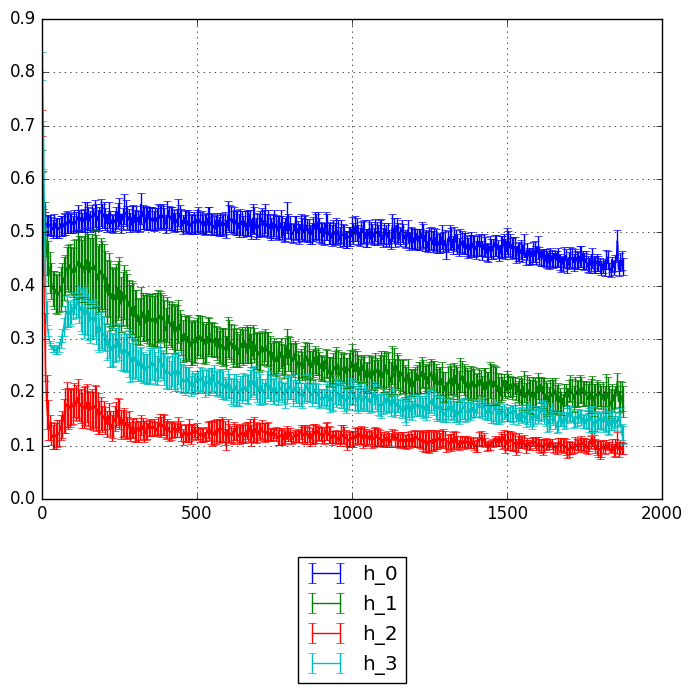
\includegraphics[scale=0.4]{gfx/l4b32_relu_xavier_identity_cnn_activations}
    		\end{figure}
    		\vfill
	\end{frame}
	\begin{frame}[t]{}{}%
		\vfill
		\begin{center}
			{$L = 4$ / Initialization: xavier / Activation: relu / Normalization: none}
		\end{center}
    		\begin{figure}
    			\centering
    			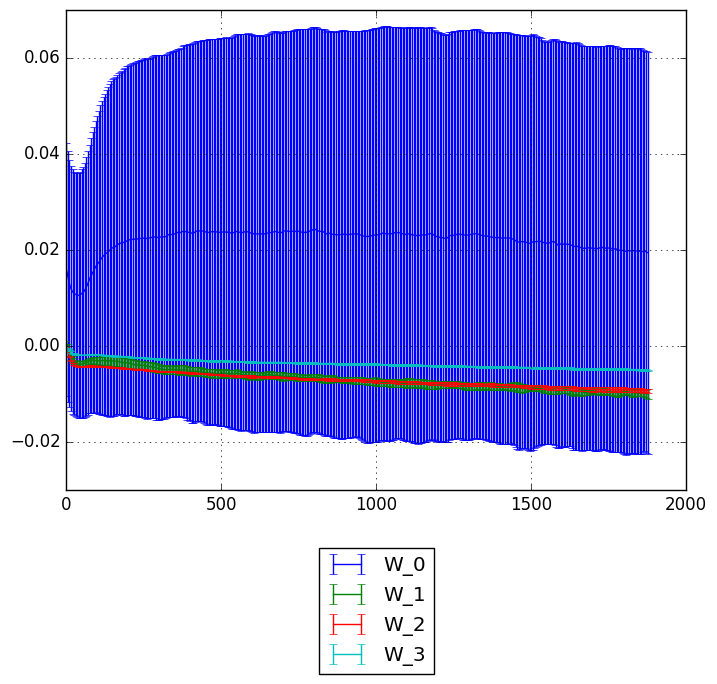
\includegraphics[scale=0.4]{gfx/l4b32_relu_xavier_identity_cnn_weights}
    		\end{figure}
    		\vfill
	\end{frame}
	
	% ReLU + Xavier + BN
	\begin{frame}[t]{}{}%
		\vfill
		\begin{center}
			{$L = 4$ / Initialization: xavier / Activation: relu / Normalization: batch normalization}
		\end{center}
    		\begin{figure}
    			\centering
    			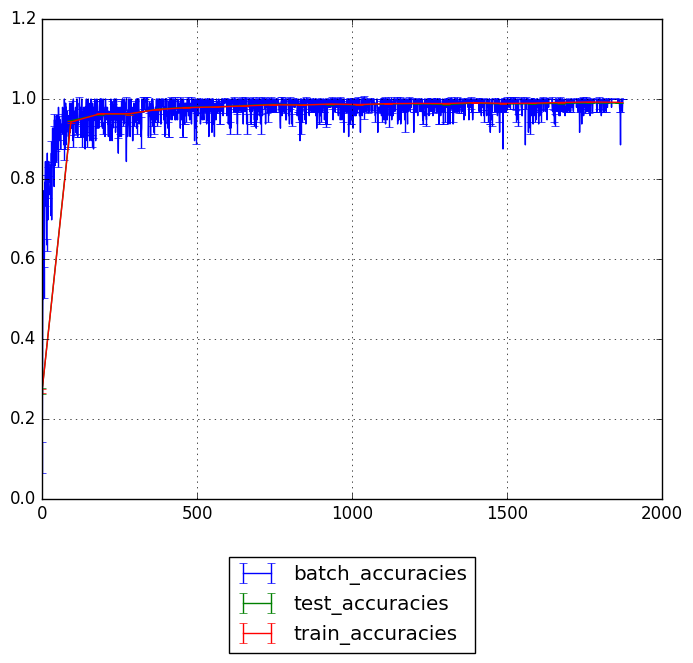
\includegraphics[scale=0.4]{gfx/l4b32_relu_xavier_batch_normalization_cnn_accuracies}
    		\end{figure}
    		\vfill
	\end{frame}
	\begin{frame}[t]{}{}%
		\vfill
		\begin{center}
			{$L = 4$ / Initialization: xavier / Activation: relu / Normalization: batch normalization}
		\end{center}
    		\begin{figure}
    			\centering
    			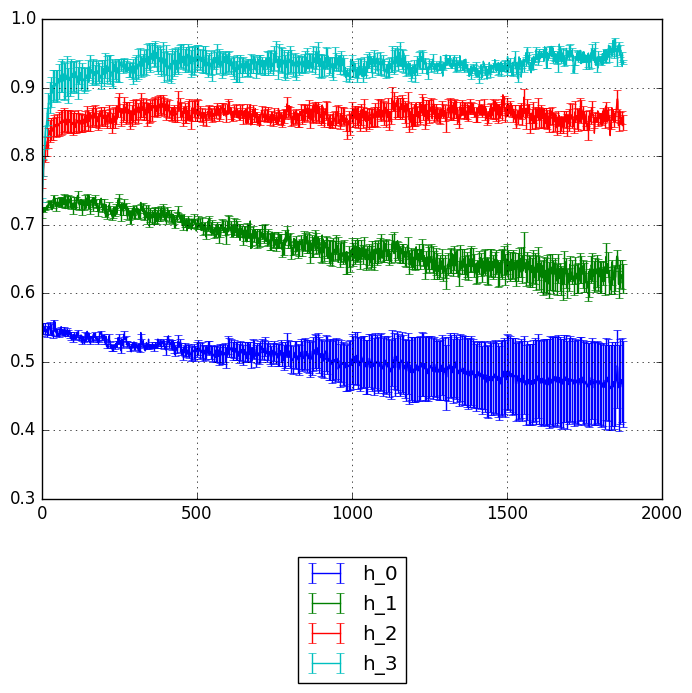
\includegraphics[scale=0.4]{gfx/l4b32_relu_xavier_batch_normalization_cnn_activations}
    		\end{figure}
    		\vfill
	\end{frame}
	\begin{frame}[t]{}{}%
		\vfill
		\begin{center}
			{$L = 4$ / Initialization: xavier / Activation: relu / Normalization: batch normalization}
		\end{center}
    		\begin{figure}
    			\centering
    			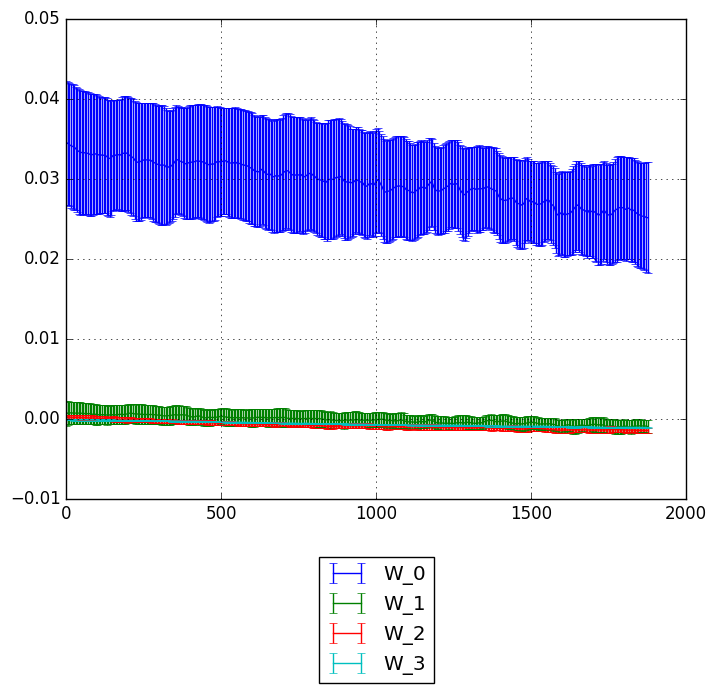
\includegraphics[scale=0.4]{gfx/l4b32_relu_xavier_batch_normalization_cnn_weights}
    		\end{figure}
    		\vfill
	\end{frame}
	
	% ReLU + Xavier + BN + 5
	\begin{frame}[t]{}{}%
		\vfill
		\begin{center}
			{$L = 5$ / Initialization: xavier / Activation: relu / Normalization: batch normalization}
		\end{center}
    		\begin{figure}
    			\centering
    			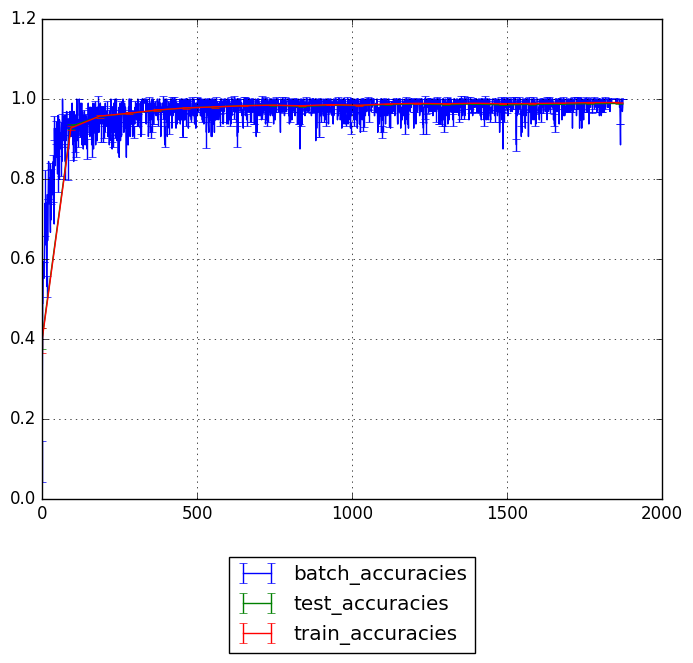
\includegraphics[scale=0.4]{gfx/l5b32_relu_xavier_batch_normalization_cnn_accuracies}
    		\end{figure}
    		\vfill
	\end{frame}
	\begin{frame}[t]{}{}%
		\vfill
		\begin{center}
			{$L = 5$ / Initialization: xavier / Activation: relu / Normalization: batch normalization}
		\end{center}
    		\begin{figure}
    			\centering
    			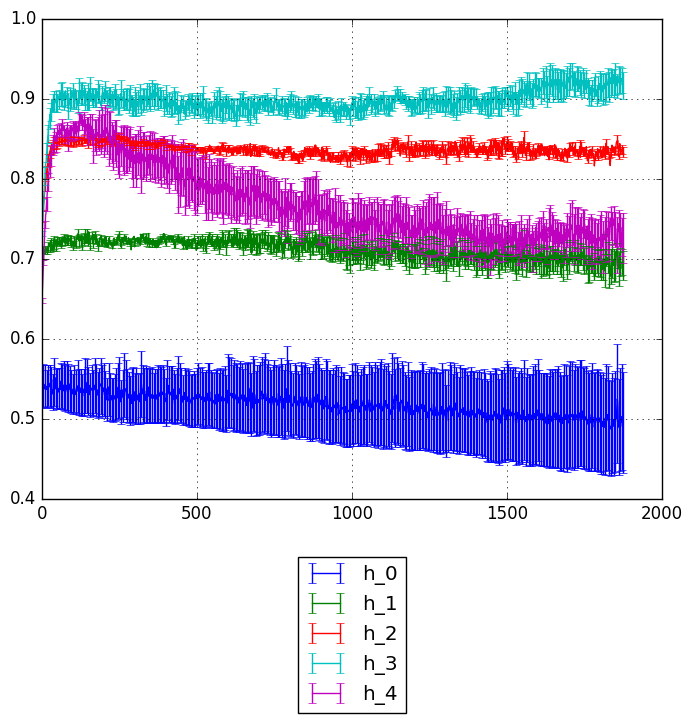
\includegraphics[scale=0.4]{gfx/l5b32_relu_xavier_batch_normalization_cnn_activations}
    		\end{figure}
    		\vfill
	\end{frame}
	\begin{frame}[t]{}{}%
		\vfill
		\begin{center}
			{$L = 5$ / Initialization: xavier / Activation: relu / Normalization: batch normalization}
		\end{center}
    		\begin{figure}
    			\centering
    			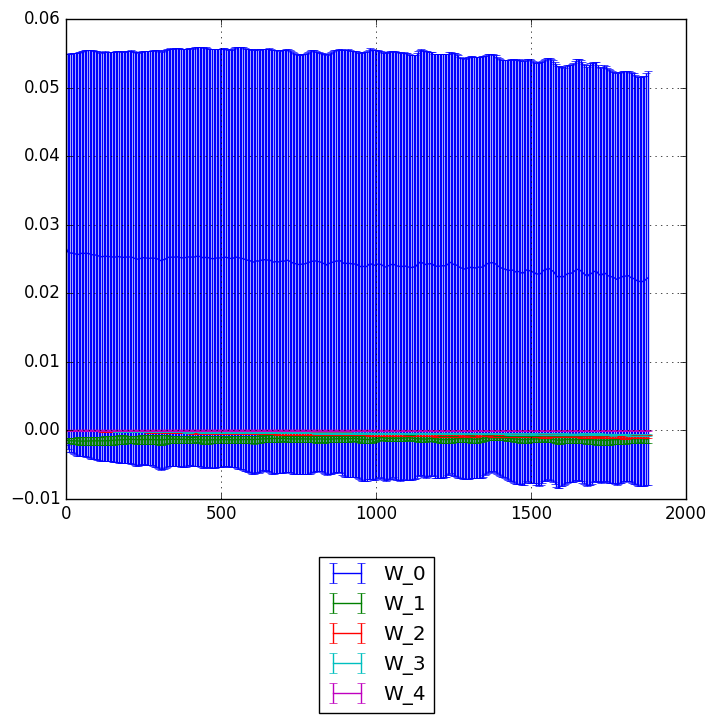
\includegraphics[scale=0.4]{gfx/l5b32_relu_xavier_batch_normalization_cnn_weights}
    		\end{figure}
    		\vfill
	\end{frame}
}	
\end{document}
